\chapter{Lepton Flavour in the Standard Model and Beyond}\label{chapter1}

% \begin{markdown}
% ---

% + Yoshi said: this is really an intro to CLFV searches for experts out of the CLFV
% field.

% + What's a muon?
% + What does the SM predict muons can/can't do
% + Historical context, motivation
%  + Why/how was the first CLFV experiment conducted?


% ---
% \end{markdown}

% v1
The Standard Model (SM) of particle physics is possibly the most successful
mathematical model of physical phenomena so far. It provides an accurate
description of all observable interactions between known elementary particles.
It yields predictions for what nature does and does not allow, and enables
physicists to examine and test the fundamental laws of the universe. It provides
a rigid framework to make theoretical predictions, from which any measured
deviations can then be interpreted as new physics.

The muon is the most sensitive probe to search for charged lepton flavour
violation. If that is observed, it will add another piece of definite evidence,
along with non-zero neutrino masses, that the SM cannot faithfully account for
all fundamental interactions.


% However before we are able to dive into the main topics, it is necessary to
% discuss the purpose of the experiment, how it emerges from the current state of
% our knowledge of elementary particle physics, and the steps taken to get there.


% v0
% Explain the SM. Something like
% The Standard Model is the theory at the heart of modern particle physics. Built
% upon special relativity and quantum mechanics, it describes the interactions
% between elementary particles and allows physicists to predict the outcome of
% interactions and decays to a previously unattainable precision. Little evidence
% so far has been able to contradict the formulation of the Standard Model,
% despite many fundamental questions remaining unanswered, such as the nature of
% dark matter, the reason for the matter-antimatter asymmetry in the universe, or
% the existence of exactly three generations of leptons and quarks.


\section{Discovery of the muon}
The first traces of muons were observed around 1937 by three experiments
investigating the nature of cosmic ray-induced particle
showers~\cite{PhysRev.51.884, PhysRev.52.1198, PhysRev.52.1003}. 
One of them was able to estimate the mass of the discovered
particle at 130 times that of the electron, around the same as the strong
force-carrying meson predicted by Yukawa in 1935~\cite{10.1143/PTPS.1.1}. 
Hence, the muon and Yukawa's particle were
originally believed to be one and the same particle. It was only a decade later, when
the meson (now called $\pi$, for primary) was observed decaying into a muon,
that the two particles were completely disambiguated~\cite{LATTES1947}.

It was the fact that the muon appeared as nothing but a heavy electron which
prompted Rabi to ask ``who ordered that?'' in response to its discovery. In
fact, even the Standard Model of today cannot give a satisfactory answer to this
question, since it does not motivate the existence of three generations of
elementary particles. As far as the SM can explain, there is no fundamental reason
for the existence of distinct flavours.

\section{The muon in the Standard Model}
% 
The SM identifies the muon as the second-generation charged lepton, meaning it
is a fermion with identical quantum numbers (aside from flavour) as the electron
and tau lepton. A muon in a vacuum can only decay through the weak force. The
diagram for muon decay, $\mu^- \rightarrow e^- +  \nu_\mu + \overline{\nu}_e$,
is shown in Fig.~\ref{fig:weak_decay}.


\begin{figure}
    \centering
    \feynmandiagram [layered layout, horizontal=a to b] {
        a [particle=\(\mu^{-}\)] -- [fermion] b -- [fermion] f1 [particle=\(\nu_{\mu}\)],
        b -- [boson, edge label'=\(W^{-}\)] c,
        c -- [anti fermion] f2 [particle=\(\overline \nu_{e}\)],
        c -- [fermion] f3 [particle=\(e^{-}\)],
    };
    \caption{Feynman diagram for the weak decay of the muon.}
    \label{fig:weak_decay}
\end{figure}

In the SM Lagrangian with massless neutrinos, none of the terms which involve
leptons allow for flavour violation. The Lagrangian is invariant under
transformations of the ${U(1)_e \times U(1)_\mu \times U(1)_\tau}$ group, and
consequently, each lepton family ($e$, $\mu$, $\tau$) has its own conserved
number which prevents a charged lepton from changing flavour without neutrinos
being involved. 

These conservation laws do not correspond to a fundamental symmetry of nature;
they are merely a feature of the SM Lagrangian and have, so far, been observed
to hold experimentally. For instance, the process ${\mu \rightarrow e +
\gamma}$, in principle allowed by kinematics, has never been observed and the
current upper limit on its branching ratio was set by the MEG experiment at
$10^{-13}$~\cite{mori2016final}.

The observation of neutrino oscillations~\cite{PhysRevLett.81.1562} means that
the three accidental flavour symmetries are not exact. This strongly
motivates a search for flavour violation among the charged leptons as well, as
any evidence for it would, together with neutrino oscillations, yield hints
about the theory lying beyond the Standard Model.

\begin{figure}
\centering
\begin{subfigure}[t]{0.45\textwidth}
    \centering
    \begin{tikzpicture}
    \begin{feynman}
    \vertex (a) {\(\mu\)};
    \vertex [right=1.5cm of a] (b);
    \vertex [right=1.8cm of b] (c);
    \vertex [right=1.5cm of c] (d) {\(e\)};
    
    \vertex at ($(b)!0.5!(c) + (0, 0.9cm)$) (n);
    \vertex at ($(b)!0.5!(c) + (0, -0.9cm)$) (w);
    \vertex [above=0.1cm of w] (wn) {\(W\)};
    \vertex [below=1.5cm of d] (g) {\(\gamma\)};
    
    \diagram* {
    (a) -- [fermion] (b)
    -- [fermion, quarter left, edge label=\(\nu_\mu\)] (n)
    -- [fermion, quarter left, edge label=\(\nu_e\)] (c),
    (b) -- [boson, quarter right] (w)
    -- [boson, quarter right] (c),
    (c) -- [fermion] (d),
    (w) -- [boson] (g),
    };
    
    \draw (n) -- (n) node {\(\times\)};
    
    \end{feynman}
    \end{tikzpicture}
    \caption{
        $\mu \rightarrow e + \gamma$
    }
    \label{fig:mu_e_nu_osc}
\end{subfigure}
\begin{subfigure}[t]{0.45\textwidth}
    \centering
    \begin{tikzpicture}
    \begin{feynman}
    \vertex (m1) {\(\mu\)};
    \vertex [right =1.5cm of m1] (m2);
    \vertex [right =1.8cm of m2] (m3);
    \vertex at ($(m2)!0.5!(m3)$) (w);
    \vertex at ($(m2)!0.5!(m3) + (0, 0.4cm)$) (wl) {\(W\)};
    \vertex at ($(m2)!0.5!(m3) + (0, 0.9cm)$) (n);
    \vertex [right =1.5cm of m3] (m4) {\(e\)};

    \vertex [below =of m1] (q1) {\(q\)};
    \vertex [below =of m2] (q2);
    \vertex [below =of m3] (q3);
    \vertex [below =of m4] (q4) {\(q\)};
    \vertex at ($(q2)!0.5!(q3)$) (qg);
    
    \diagram* {
    (m1) -- [fermion] (m2)
    -- [fermion, quarter left, edge label=\(\nu_\mu\)] (n)
    -- [fermion, quarter left, edge label=\(\nu_e\)] (m3),
    (m2) -- [boson] (w)
    -- [boson] (m3)
    -- [fermion] (m4),
    (q1) -- [fermion] (q2)
    -- (q3)
    -- [fermion] (q4),
    (w) -- [boson, edge label=\(\gamma\)] (qg),
    };

    \draw (n) -- (n) node {\(\times\)};
    
    \end{feynman}
    \end{tikzpicture}
    \caption{
        $\mu+N \rightarrow e + N$
    }
    \label{fig:mu-e_conv_SM}
\end{subfigure}
    \caption{
        Feynman diagrams of processes allowing charged lepton flavour
        violation in the SM extended with neutrino masses. Although these
        processes enable CLFV, their branching ratios are heavily suppressed to
        unobservable levels because of the lightness of
        neutrinos compared to the weak scale~\cite{BERNSTEIN201327}.}
\end{figure}

The fact that neutrinos can change flavour allows a process such as shown in
Fig.~\ref{fig:mu_e_nu_osc} to occur, which gives rise to a non-zero rate for
${\mu \rightarrow e + \gamma}$. However, the branching ratio calculated for this
process using the upper limit on neutrino masses is given by:
\begin{equation}\label{eq:br_meg}
\mathcal{BR}(\mu \rightarrow e + \gamma) = \frac{3\alpha}{32\pi} \left|\ \sum_{i=2, 3} U^*_{\mu i} U_{e i} 
\frac{\Delta m^2_{i1}}{M^2_W}  \ \right| ^2 \approx 10^{-54},
\end{equation}
where $U$ is the PMNS matrix, $\Delta m^2_{ij}$ is the mass-squared difference between the
$i$-th and $j$-th neutrino mass eigenstates, and $M_W$ is the $W$-boson
mass~\cite{BERNSTEIN201327}.
Hence, any evidence that the ${\mu \rightarrow e + \gamma}$ process occurs at a higher
rate than given by Eq.~\ref{eq:br_meg} would indicate that another channel,
involving charged lepton flavour violation, is responsible.

\section{Charged lepton flavour violation}

The processes involving muons which are most sensitive for probing charged
lepton flavour violation (CLFV) are ${\mu \rightarrow e + \gamma}$, ${\mu
\rightarrow e+e+e}$ and ${\mu + N \rightarrow e + N}$~\cite{BERNSTEIN201327}.
Observing CLFV with any one of them would corroborate the fact that the SM
Lagrangian is incomplete, as is now known from neutrino oscillations. Measuring
CLFV in two or more processes would then help us to determine which --- if any
--- of the many theorised models for new physics is realised in nature.


CLFV has been sought after ever since the muon's discovery: the first
investigation of whether nature allows $\mu \rightarrow e + \gamma$ was done in
1948~\cite{PhysRev.73.257}. A multitude of experiments followed, but none so far
have been able to find a signal. Fig.~\ref{fig:clfv_upper_limit} shows
experimentally estimated upper limits on the branching ratios of $\mu
\rightarrow e\gamma$, $\mu\rightarrow eee$ and $\mu N \rightarrow e N$ over
time, since the first experiment and into the next decade. As
higher and higher sensitivities are required, experiments must be able to
produce a muon source which is more and more intense while demonstrating a
precise control over every source of background. The next generation of
CLFV-seeking precision experiments, which consists of MEG II, Mu3e, COMET and
Mu2e, aims to be 10 to \numprint{10000} times more sensitive than the last
generation.

\begin{figure}
    \centering
    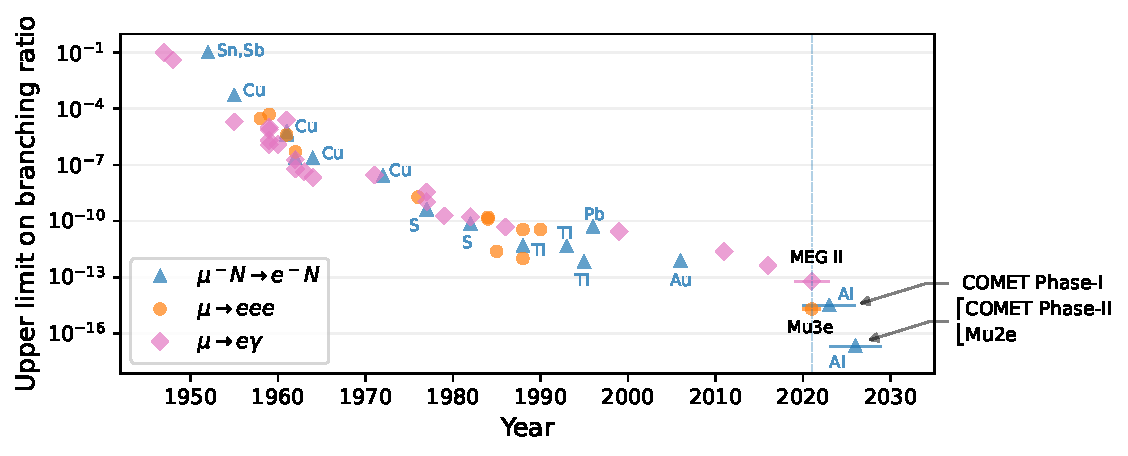
\includegraphics[width=\textwidth]{chapter1/clfv_upper_limit_v2.pdf}
    \caption{
        90\%-confidence upper limit on the branching ratio of three charged
        lepton flavour-violating processes over time. 
        The target material $N$ is indicated for $\mu$--$e$ conversion experiments.
        Past experiment results
        were tabulated in~\cite{BERNSTEIN201327}. Future data points are the
        expected sensitivities quoted in the MEG II~\cite{Baldini2018},
        Mu3e~\cite{ARNDT2021165679}, COMET
        Phase-I~\cite{the_comet_collaboration_comet_2020} and
        Mu2e~\cite{bartoszek2015mu2e} design reports.
    }
    \label{fig:clfv_upper_limit}
\end{figure}

\subsection{Muon to electron conversion}
% mu-e conversion
Muon to electron conversion is the neutrino-less decay of a muon bound to an
atomic nucleus:
$$
\mu^- + N(A, Z) \rightarrow e^- + N(A, Z),
$$
where $A$ is the mass number and $Z$ the atomic number.
Similarly to $\mu\rightarrow e+\gamma$, this process is allowed in the SM
extended with massive neutrinos via the diagram shown in
Fig.~\ref{fig:mu-e_conv_SM}, but suppressed to an experimentally
unreachable level.

In order to search for this process, muons must be stopped in matter to form
muonic atoms. Initially stopped in the outer atomic layers, the muon electromagnetically
cascades down to the $1s$ orbital and gets in range of the nucleus. In the SM,
it is then allowed to either decay in orbit: ${\mu^- + N(A, Z) \rightarrow e^- + \nu_\mu +
\overline{\nu}_e + N(A, Z)}$; or it can be captured by the nucleus via a $W$ exchange: ${\mu^- +
N(A, Z) \rightarrow \nu_\mu + N(A, Z-1)}$. 
% Quote branching ratios?
The reaction is called \emph{coherent} if it leaves the nucleus in its ground
state~\cite{CHIANG1993526}. In this case, the energy of the products is more
easily calculated.

In a coherent $\mu$--$e$ conversion, the energy of the outgoing electron is
$$
E_e = m_\mu - E_B - E_R,
$$
where $E_B$ is the binding energy and $E_R$ is the recoil energy.

% Energy level
% SM backgrounds






The COMET experiment will search for muon to electron conversion in muonic
aluminium atoms, $\mu^- + \mathrm{Al} \rightarrow e^- + \mathrm{Al}$.




% Since 1948~\cite{PhysRev.73.257}, searches for ${\mu \rightarrow e + \gamma}$
% have demonstrated that it does not occur at any observable rate: the current
% upper limit on its branching ratio measured by the MEG experiment is
% $10^{-13}$~\cite{mori2016final}.

% In the quark sector, generations can mix via weak interactions: the
% CKM matrix accurately describes how strongly each quark flavour couples
% to the others. %~\cite{PhysRevLett.10.531, 10.1143/PTP.49.652}.
% For leptons on the other hand, it is
% only through neutrino oscillations, discovered by the Super-Kamiokande
% experiment~\cite{PhysRevLett.81.1562}, that flavours have been observed to mix. 
% Flavour-changing neutrino oscillations allow a new channel for ${\mu \rightarrow
% e + \gamma}$, shown in Fig.~\ref{fig:mu_e_nu_osc}. 




% Allowed and forbidden decays

% g-2 measurement
\cite{PhysRevLett.126.141801} % g-2

% Is lhc-b related here? Lepton univ?
\cite{Aaij2022}% lhc-b R_K




\section{Models}
Quark generations are known to mix (CKM).
Neutral leptons (neutrinos) are known to mix (PMNS, osc).
Charged leptons have never been seen to mix. Why?

